\chapter{Introduction}
\label{cha:intro}


% SECTION 1

\section{Microbial communities: composition 
% (\textit{who})
, functions 
% (\textit{what}) 
\& intections 
% (\textit{how})
}
   % WHO : DIVERSITY 
   \subsection{Microbial diversity: life under extraordinary conditions}
   \label{subsec:microbial_diversity}

      Microbes are considered to be omnipresent in the 
      various ecosystems on Earth~\citep{falkowski2008microbial}.
      It was only until recently, \citeyear{belilla2019hyperdiverse}, that scientists discovered for the first time 
      a place on Earth where no microbial forms of life are present~\cite{belilla2019hyperdiverse}.
      Extremely low pH, high salt and high temperature had to be 
      at the same place at the same time to stop microbes.
      However, microbes are not just abundant but 
      exceedingly variant too.
      \citeauthor{locey2016scaling} using a unified scaling law
      and a lognormal model of biodiversity, 
      estimated microbial diversity at about 1 trillion species~\cite{locey2016scaling}.
      However, despite the extensive studies of the scientific community, 
      less than 1\% of the microbial species on Earth have been identified~\cite{isme}.
      
      Microbes are distinguished by multiple properties.
      Based on their morphology microbes can be spherical (cocci), rod-shaped (bacilli),
      arc-shaped (vibrio), and spiral (spirochete)~\cite{dunlap2001microbial}.
      Based on their metabolic characteristics, microbes are further distinguished. 
      More specifically, according to their \textit{energy source}, a microbe
      can either oxidate inorganic compounds (\textbf{chemotrophs}) or sunlight (\textbf{phototrophs}).
      Similarly, microbes can use CO$_2$ (\textbf{autotrophs}) as their \textit{carbon source},
      or organic compounds (\textbf{heterotrophs}) or both (\textbf{mixotrophs}).
      Finally, based on their \textit{electron source} 
      microbes are distinguished bewtween those using inorgarnic compounds (\textbf{lithotrophs}) and those using organic compounds (\textbf{organotrophs})~\cite{madigan2018brock}.
      Microbial taxa combine combinining alternatives of the aforementioned categories 
      shape a range of microbial profile of all the possible combinations; for example      \textbf{chemolithoautotrophic} bacteria, 
      e.g. nitrifying and sulfur-oxidizing bacteria, as well
      as \textbf{photoautotrophic} bacteria, 
      e.g. purple bacteria and Green sulfur bacteria. 
      Finally, microbia taxa can also be disinguished by their various ecological distributions and activities, 
      and by their distinct genomic structure, expression, and evolution~\cite{dunlap2001microbial}. 

   % WHAT : FUNCTIONAL POTENTIAL
   % \if 0
   \subsection{Functional diversity: shaping the conditions of life}
   \label{subsec:functional_diversity}
   % \fi 
      However, it is not only the number of microbial taxa and their massive biomass that
      make the study of microbial communities essential; 
      it is mostly their functional potentials. 
      Life on Earth would not be as we know it, if existed at all, if it was not for the 
      microbes and their long contribution on ensuring life-supporting conditions. 
      Nevertheless, these are the \textit{biological machines responsible for planetary
      biogeochemical cycles}~\cite{falkowski2008microbial}; meaning that biogeochemical cycling 
      to a global extent
      is powered by the metabolic processes of the microbial taxa~\cite{louca2016decoupling}. 
      In Figure~\ref{fig:co2} the contibution of microbial communities 
      in the cycle of CO$_2$ is shown. 

      \begin{figure}[h]
         \centering
         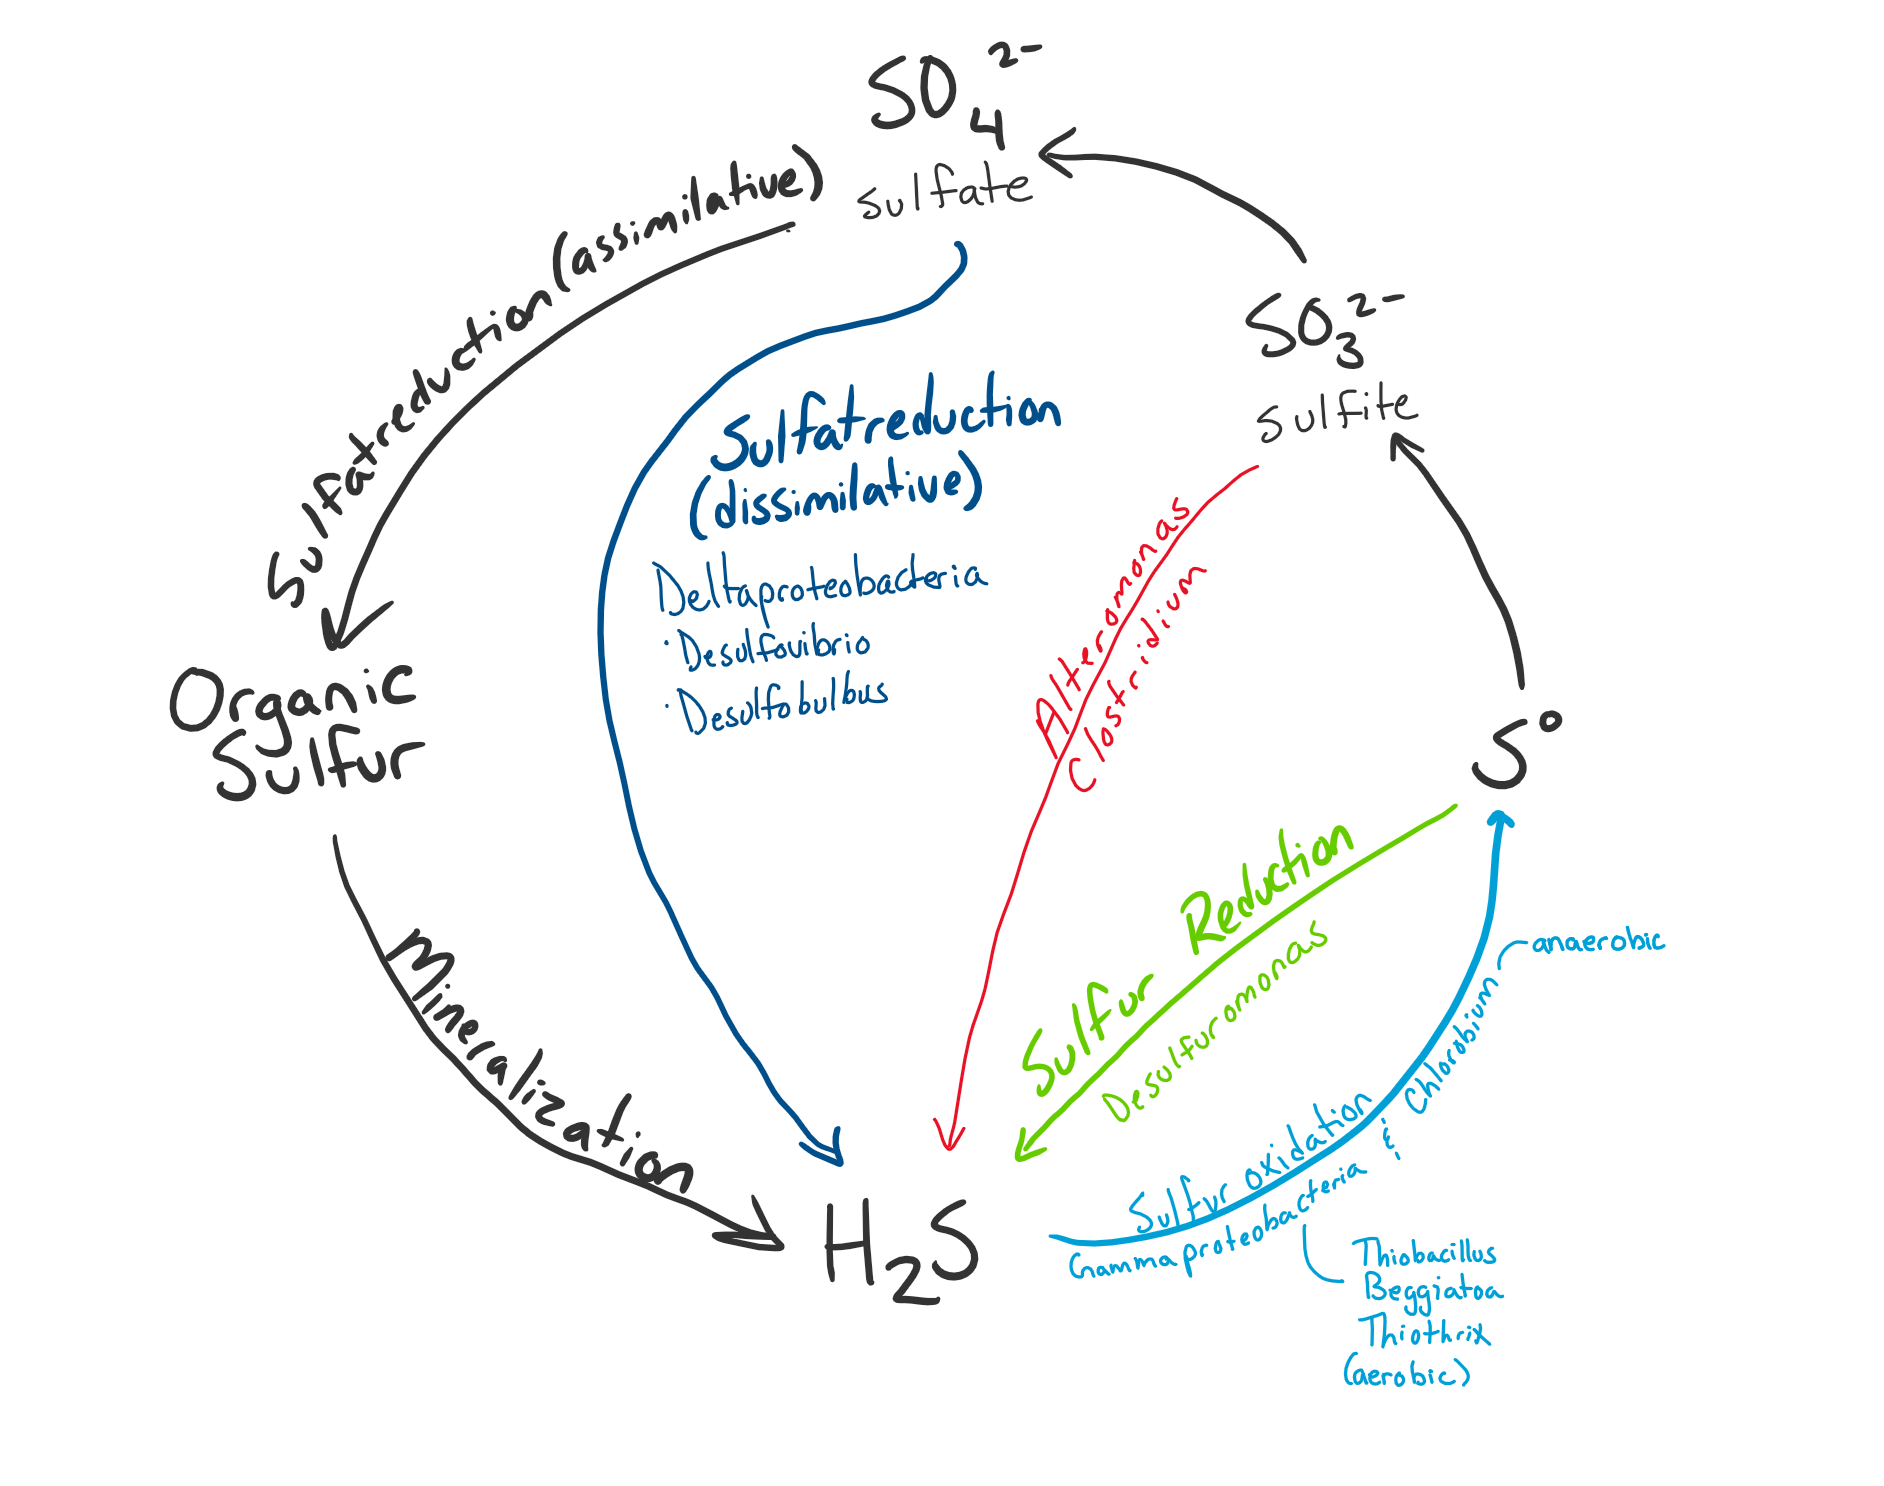
\includegraphics[width=0.65\textwidth]{figures/Sulfur_Cycle_for_Hydrothermal_Vents.png}
         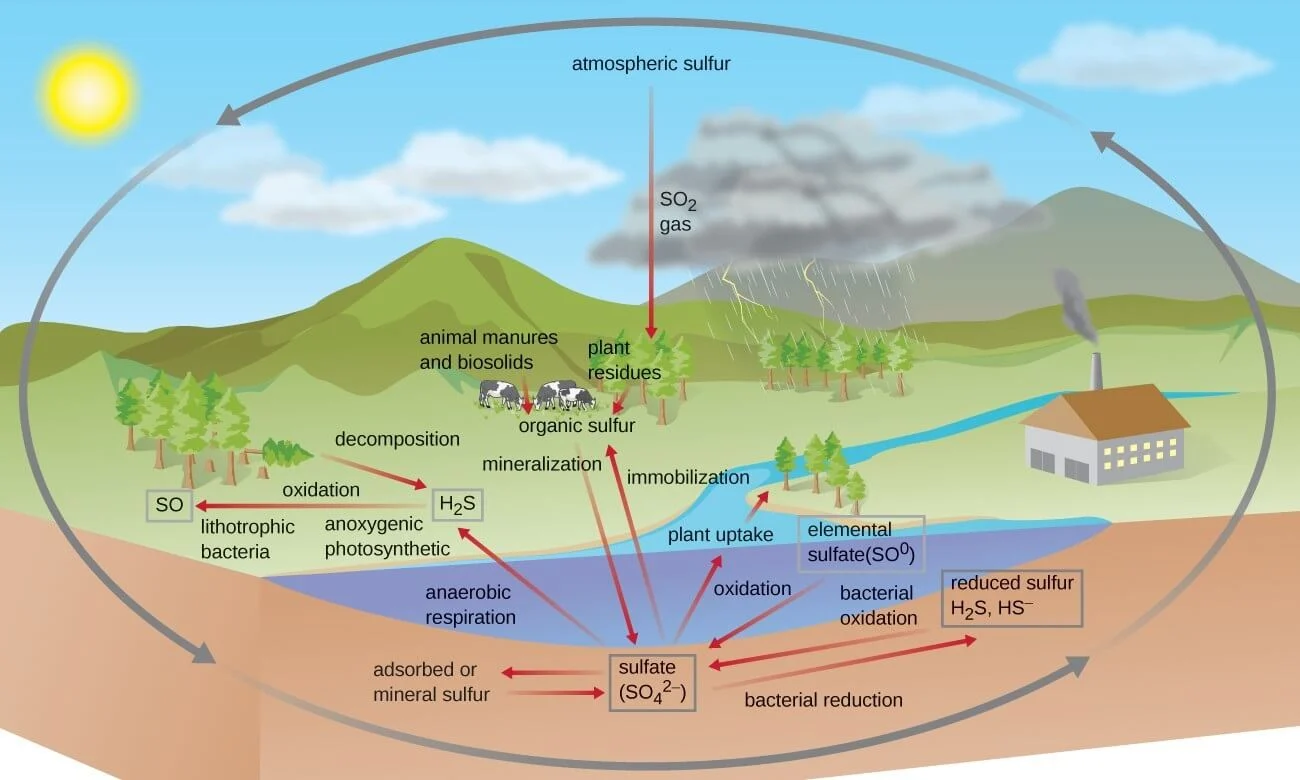
\includegraphics[width=0.95\textwidth]{figures/sulfur_village.png}
         \caption[The cycle of S and the role of microbial communiites]{
            The cycle of sulfur (S) (up) and the contribution of microbial communities on it (down, image source: \href{https://openstax.org/resources/3002d0fba25221d24455917117482a079a11f321}{OpenStax}).
            % Marine microbial communities contribute to CO$_2$ sequestration, nutrients recycle and thus to the release of CO$_2$ to the atmosphere. 
            % Soil microbial communities decomposers organic matter and release nutrients in the soil 
            % from \citep{cavicchioli2019scientists} doi: \href{https://doi.org/10.1038/s41579-019-0222-5}{10.1038/s41579-019-0222-5}, under \href{http://creativecommons.org/licenses/by/4.0 license}{Creative Commons Attribution 4.0 International License}
         }
         \label{fig:co2}
      \end{figure}

      The biological fluxes of most of the major elements (i.e., carbon, hydrogen, oxygen, nitrogen and sulfur) required
      for any biological macromolecule,
      are driven largely
      by microbially catalyzed, thermodynamically constrained redox reactions~\cite{falkowski2008microbial}. 
      Phosphorus the last of the 6 fundamental elements for life, is also included in the metabolic pathways catalyzed by microbes. 
      Thus, microbial communities consist of hundreds or even thousands of metabolically diverse strains and species~\cite{leventhal2018strain},
      and their functions
      and determine the fitness of most organisms on Earth. 
      In case of human health, specific microbial enzymatic pathways and molecules necessary for health promotion have been well known.
      Some of these "beneficial factors" are already known for probiotics and species in the human microbiome~\cite{marco2021defining}.


      % MICROBIAL ECOLOGY and OPEN QUESTIONS 
      % \if 0
      % \myparagraph{Microbial Ecology}
      % \fi
      \paragraph{Microbial Ecology} focuses on the study of the following interactions: 
      \begin{itemize}
         \setlength\itemsep{0.05em}
         \item those between microbial taxa and their environment
         \item those among the various microbial taxa present in a community, and
         \item those between microbial taxa and their host~\cite{isme}
      \end{itemize}

      Microbial ecologists also investigate the role of microbial taxa in 
      biogeochemical cycles~\cite{falkowski2008microbial} and their interaction 
      with anthropogenic effects e.g. pollution and climate change~\cite{cavicchioli2019scientists}.

      Even though HTS has allowed a massive extension of our knowledge in  
      specific enzymatic reactions that regulate these pathways the rules that determine 
      the assembly, function, and evolution of these microbial communities remain unclear. 
      Thus, both in case of environmental and human
      the underlying mechanisms for how microbial assemblages work and affect their environment, remain to be discovered.
      Understanding the underlying governing principles is central to microbial ecology~\cite{giri2021metabolic} and crucial for designing microbial consortia for biotechnological~\cite{giri2020harnessing} or medical applications~\cite{kong2018designing}.

      Studies such as the one of~\citeauthor{louca2016decoupling}
      have opened new frontiers in our understanding on microbial assemblages. 
      After building metabolic functional groups and assigning more than 30,000 marine 
      species to these groups,~\citeauthor{louca2016decoupling} showed 
      that the distribution of these functional groups were influenced by environmental 
      conditions to a great extent, shaping \textit{metabolic niches}.
      At the same time though, the taxonomic composition within individual functional groups
      were not affected by such environmental condintions~\cite{louca2016decoupling}.

   % MICROBIAL INTERACTIONS INTRO
   % \if 0
   \subsection{Ecological interactions in microbial communities}
   \label{subsec:ecol_interactions}
   % \fi
      Moreover, to elucidate how these assemblages work the biotic interactions have to be 
      considered too. 
      Microbial interactions play a fundamental role in deciphering the underlying mechanisms that govern ecosystem functioning \cite{braga2016microbial, faust2012microbial}. 
      Microbes secrete costly metabolites (called \textbf{byproducts}) to their environment, 
      which other microbes can absorb and exploit~\cite{pacheco2019costless}.
      By exchanging metabolic products, mostly as there are also other ways of interactions 
      e.g. quorum sensing, microbial taxa establish various interactions. 
      
      The interaction between two taxa can either be nutral or 
      positive / negative.
      In case of a positive interaction, 
      there is a case where both taxa benefit one from another.
      This \textit{win-win} relationship is called \textbf{mutualism} (or "cooperation")
      and it can be a result of
      \textit{cross-feeding}, in which two species exchange metabolic products~\cite{faust2012microbial}.
      Such is the case in biofilms where multiple bacterial taxa are working together  
      building a structure that provides them antibiotic resistance~\cite{santos2019evolutionary}.
      There is also the case where only one of the two taxa
      benefits without helping or harming the other; 
      this interaction is called \textbf{commensalism}~\cite{faust2012microbial}. 
      For example, \textit{Nitrosomonas} oxidize ammonia (NH$_3$) into nitrite (NO${_2}^{-}$), so  
      \textit{Nitrobacter} can use it to obtain energy and oxidize it into nitrate (NO${_3}^{-}$)~\cite{laanbroek2002nitrite}.
      Such interactions are quite common in microbial communities.

      \begin{figure}
         \centering
         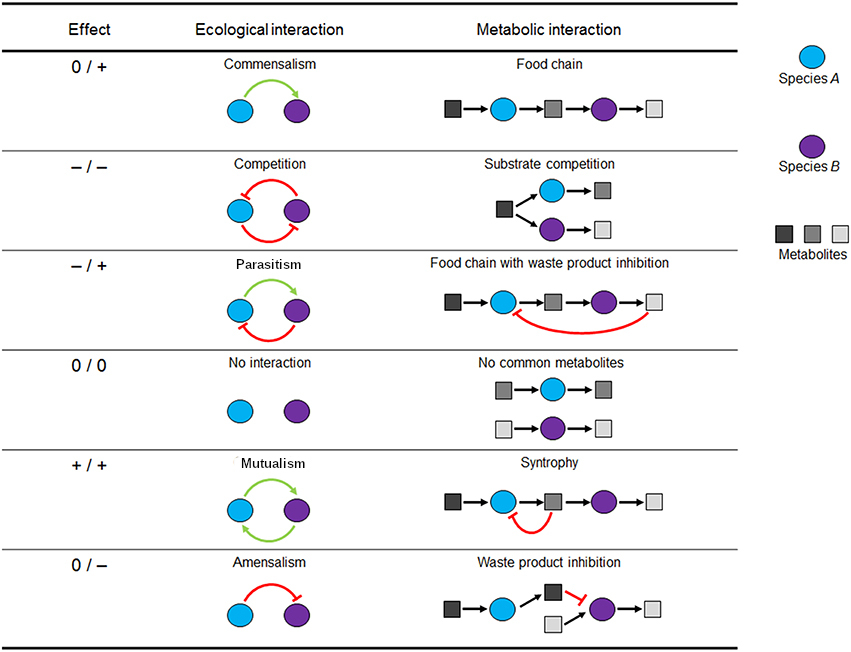
\includegraphics[width=.9\textwidth]{figures/interaction_types.jpg}
         \caption[Microbial interactions types]{Microbial interaction types along 
         with their corresponding metabolic ones.
         Due to certain metabolic interactions, two taxa may have a positive, a negative
         or a nutral effect one another. 
         Figure based on \cite{perez2016metabolic}}
         \label{fig:micro-inter-types}
      \end{figure}

      In case of a negative interaction, can harm each other either way (\textbf{compe-tition}). 
      That is the case between 
      \textit{Listeria monocytogenes} and \textit{Lactococcus lactis} in the study of~\citeauthor{freilich2010large} where their resource competition is high enough
      contributing to their non-overlapping existence~\cite{freilich2010large}.
      Moreover, similarly to commensalism, 
      there is also the case when a taxon has a negative affect on the other
      without getting any harm (\textbf{amensalism}). 
      Such is the case for \textit{Acidithiobacillus thiooxidant} that produces
      sulfuric acid (H$_2$SO$_4$) by oxidation of sulfur~\cite{bobadilla2013stoichiometric} which is responsible for lowering of pH in the culture media which inhibits the growth of most other bacteria~\cite{jin2018ph}.
      Finally, one of the taxa may have a positive affect (host) on the other, but the 
      latter (parasite) can be harmful to its benefator (\textbf{parasitism})~\cite{faust2012microbial}. 
      There are multiple cases of parasitism in real-world communities; 
      specis of the genus \textit{Bdellovibrio} for example, are parasites of other (gram-negative) bacteria~\cite{stolp1979interactions}.

      Apparently, the environmental conditions affect the ecological interactinos to a
      great extent. 
      A pair of taxa may be competitors in one case but have a nutral intrection in another one. 
      In addition, evolutionary processes may change certain interactions; 
      for example moving from commensalism to parasitism~\cite{parmentier2016commensalism}.
      Both ecological and environmental interactions 
      play a part in the composition and the functional potential of 
      microbial assemblages. 


% SECTION 2

\section{High Throughput Sequencing in Microbial Ecology}

      % SUBSECTION 1.1.2 
   \subsection{'Omics methods to access the \textit{who} and the \textit{what}}
   \label{subsec:omics}
      To discover the microbial taxa present in a sample, scientists have 
      explored multiple ways throught the years. 
      Only a particularly limited proportion of the microbial species 
      can be cultured~\cite{steen2019high}.
      Therefore, monocultures and enrichment cultures allow us to observe 
      only a small fraction of the actual diversity. 
      As a consequence, other methods for the taxonomic identification of theses
      species are required.
      Based on molecular characteristics of the microbial taxa, 
      over the last decades, a series of methods have been developed. 
 
      Moving from single species to assemblages, molecular-based identification and functional 
      profiling of communities has become available through marker (metabarcoding), 
      genome (metagenomics), or transcriptome (metatranscriptomics) sequencing from environmental 
      samples \citep{goldford2018emergent}. 
      To a great extent, these methods address the problem of how to produce and get access 
      to the information on different biological systems and molecules.

      In case that the taxonomic assesment of a sample is the aim of a study, 
      \textit{metabarcoding} (amplicon-targeted metagenomics) and \textit{shotgun metagenomics} can be used as alternative options. 
      Metabarcoding studies are common, well-established, cheaper and less computationally demanding than shotgun metagenomics~\cite{bell2021comparing}. 
      Its primary drawbacks are the limited information present in the short barcoding sequence and the possible taxonomic bias arising from differential efficiency of PCR primer pairing in different species~\cite{blazewicz2013evaluating}. 
      On the other hand, shotgun metagenomics offers a better taxonomic resolution at the species level by obtaining information from random sampling of virtually all genomic regions, and can address microbiome metabolic functions and entire biochemical pathways~\cite{sharpton2014introduction}. 
      Unfortunately, it requires higher sequencing coverage and, consequently, more complex and demanding downstream bioinformatic analysis~\cite{laudadio2018quantitative}. 
      Nevertheless, it has recently been suggested that shotgun metagenomics provides a deeper characterisation of microbiome complexity that metabarcoding recently enabling to profile up to the level of strains, whose non-core genome is responsible for crucial functional differences within the same species, as the fundamental units of the community~\cite{davila2019review, clooney2016comparing, segata2018road}.       
      
      Targeting community composition and functional profiles in several ecological niches, 
      microbial ecologists produce vast 
      amount of sequencing data~\cite{harrison2021european}.
      These approaches enable the study of ecosystems with no prior knowledge of the resident species, 
      while at the same time a number of challenges for their management and bioinformatics analysis is rising. 
   \subsection{Bioinformatics challenges in the analysis \& management of HTS data}
   \label{subsec:hts_chal}

      Moving from raw data to taxonomic and functional profiles of a microbial community comes with high computational costs, especially in the case of metagenome studies~\cite{yang2021review}.
      Sequence pre-processing, assembly, classification, and functional annotation consist of several steps the most of which a significant number of algorithms or/and software tools are available~\cite{breitwieser2019review, roumpeka2017review}. 
      Tailoring each tool's execution parameters to reflect each experiment's idiosyncrasy is vital for legitimate findings, yet it makes analyses of metagenomic data even more complex. 

      In addition, there are several challenges on the bioinformatics analysis \textit{per se}.
      \textit{Taxonomy assignment} in both amplicon- and shothun metagenomics studies 
      has several issues to meet~\cite{simon2019benchmarking};
      the taxonomy of microbes is a challenge per on its own~\cite{parks2020complete}.

      In amplicon studies, among the most major issues is the one of the abundances of the
      taxa found~\cite{fonseca2018pitfalls, balint2016millions} as well as the presence of pseudogenes~\cite{song2008many}.
      In the first case, 
      % a number of 
      issues such as  
      % \begin{itemize}
      %    \setlength\itemsep{0.05em}
         % \item 
      the usually unknown number of markere gene copies per cell in the various taxa,
         % \item 
      PCR - related biases such as primer-template mismatches, length difference of amplicon, artificial base changes, chimeric molecules 
         % \item 
      and library preparation - related issues such as chimera formation by the mix of amplicons from different samples
      % \end{itemize}
      makes hard for the method to have robust quantitative results~\cite{balint2016millions}. 
      Reads on the other hand resulting from pseudogenes or/and highly divergent nuclear mitochondrial pseudogenes (NUMTS), nonfunctional copies of mtDNA in the nucleus that have been found in major clades of eukaryotic organisms~\cite{bensasson2001mitochondrial}, 
      can lead either to false positive taxonomic hits or to non-hits at all,
      adding extra noise to the amplicon results returned.

      In shotgun metagenomics studies there are also several challenges. 
      Meta-genome \textit{assembly} comes with a great number of challenges. 
      Due to the uneven (and unknown) representation of the different organisms within a metagenomic mixture, simple coverage statistics can no longer be used to detect the repeats, while unrelated genomes may contain
      nearly-identical DNA (inter-genomic repeats) representing, for example, mobile genetic elements~\cite{ghurye2016focus}.
      At the same time, \textit{binning} is a rather tricky step too; 
      several algorithms have been developed to address it~\cite{yue2020evaluating}
      while pproaches combining the output of individual algorithms have been introduced too~\cite{song2017binning_refiner}.


      The vast amounts of data that come with metagenomic studies and the computational complexity for implementing multiple steps mentioned earlier imply immense computational requirements for their analysis that usually exceed the capacity of a standard personal computer~\cite{merelli2014managing}. 
      % 
      % Therefore, several pipelines were established to address the challenges of the bioinformatics analysis of metagenomes. 
      % In addition, as such analyses exceed the capacity of a standard personal computer, it is essential for the researchers to ensure access to  
      % computing infrastructures that will support their needs.
      % Computing infrastructures may range from a local server of an individual lab to High-Performance Computing (HPC) or/and cloud solutions adopted at the (inter)national level, such as the \href{https://eosc-portal.eu}{EOSC} and 
      % \href{https://www.embassycloud.org}{EMBL-EBI Embassy Cloud}. 
      % 
      % The swift pace of establishing new algorithms and software as well as new versions of already published ones makes software versioning an essential issue for FAIR microbiome bioinformatics analyses. 

      \paragraph{For HTS data to be available }
      to the scientific community for further exploitation,
      it is required to be accompanied by
      comprehensive metadata~\cite{vangay2021microbiome}. 
      The potential of HTS data is revealed when they are available to the community; 
      this way studies that could never been performed
      by individual researchers, labs or institutes are now possible. 
      This way, 
      a single researcher can now investigate
      how a certain environmental type reacts in response to an environmental 
      variable by making use of hundreds of metagenomic samples 
      that fulfill the criteria of his/her study.
      Finding data of interest however, can be particularly difficult.
      This is so because of a combination of reasons.
      HTS data can be particularly heterogeneous based on both the data generation and the data processing methods used. 
      However, it is mostly the vague or even absent metadata accompanying the HTS data set several limitations in their re-usage~\cite{hu2022challenges}. 

      The concept of FAIR data (Findability, Accessibility, Interoperability \& Reuse)
      and the \href{https://www.go-fair.org/fair-principles/}{FAIR principles}\footnote{\href{https://www.go-fair.org/fair-principles/}{https://www.go-fair.org/fair-principles/}}
      along with community - driven standards and resources such as 
      the \href{https://gensc.org/}{Genomic Standards Consortium (GSC)}\footnote{\href{https://gensc.org/}{https://gensc.org/}},
      the Minimal Information about any Sequence (MIxS)~\cite{yilmaz2011minimum, yilmaz2011genomic}
      and the \href{https://microbiomedata.org/metadata/}{National Microbiome Data Collaborative (NMDC)}\footnote{\href{https://microbiomedata.org/metadata/}{https://microbiomedata.org/metadata/}}~\cite{wood2020national}
      aim to address these challenges~\cite{wilkinson2016fair}.



\section{Data integration in the service of microbial ecology}


   \subsection{Moving from \textit{partial} to more \textit{complete} data interpretation}

      Over the last decades, based on
      computational and mathematical analysis and modeling,
      and by exploiting interdisciplinary data and knowledge, 
      Systems Biology focuses on complex interactions within biological systems~\cite{tavassoly2018systems}.
      The more data becoming available from all the different levels
      of hierarchy of life, the more feasible for scientists to 
      move from reductionism to more holistic approaches 
      for interpreting how the properties of a system emerge~\cite{noble2008music}.

      Microbial ecology as a field would have not been the same if it was not 
      for resources such as 
      Integrated Microbial Genomes (IMG) and GOLD~\cite{chen2021img}, 
      SEED and the Rapid Annotation of microbial genomes using Subsystems Technology (RAST)~\cite{overbeek2014seed}, 
      Pathosystems Resource Integration Center (PATRIC),
      ~\cite{zhulin2015databases}
      and many more that thousands of researches use in their every day work. 
      All these approaches, regardless on what they focus, they are all based on data aggregation and data integration approaches. 
      \textit{Data aggregation} denotes the gathering of data from diverse sources
      in a certain scheme that will allow them to be used as a combined dataset for 
      furthere analysis~\cite{simpson2010secure}. 
      In case of microbial ecology, that means that data focusing on the genetic 
      information can be combined with phenotypical data or even with environmental and 
      ecological data.
      \textit{Data integration} on the other hand, is the process of combining everything
      retrieved on the data aggregation step, 
      to get a summarization and unified view of all the accumulated data~\cite{schneider2012teaching}.
      Such summarizations may lead researhcers to new hypotheses that 
      in turn, will be tested through new experiments (Figure~\ref{fig:data_int}).


      \paragraph{Data integrations comes with great challenges.}

      Apparently, data integration methods are based on the existance of primary databases. 
      Each of these database resources come with its own assumptions and schemas. 
      Therefore, it is not a straight-forward task to recognize or assign and maintain 
      the correct names of biological entities across the various databases~\cite{stein2003integrating}.
      Taxonomy is quite an indicative example. 
      As there is no a global taxonomy system, even the species name can be a 
      great challenge in such approaches; how to retrieve information about a species
      that does not have the same name on the various databases to integrate? 
      Thereofre, retrieving and mapping entities can be rather complex.  
      Similarly to taxonomy, most biological databases are constantly changing. 
      Thus, integration approaches need to be periodically so the always keep updated~\cite{stein2003integrating}.
      In addition to the heterogenety of the data \textit{per se},
      further challenges that make data integration even harder in case of biological data,
      is the lack of unique standards~\cite{triplet2011systems}.
      In the case of HTS data, great efforts to address this challenge have been 
      made (see Section~\ref{subsec:hts_chal}).

      \begin{figure}[!h]
         \centering
         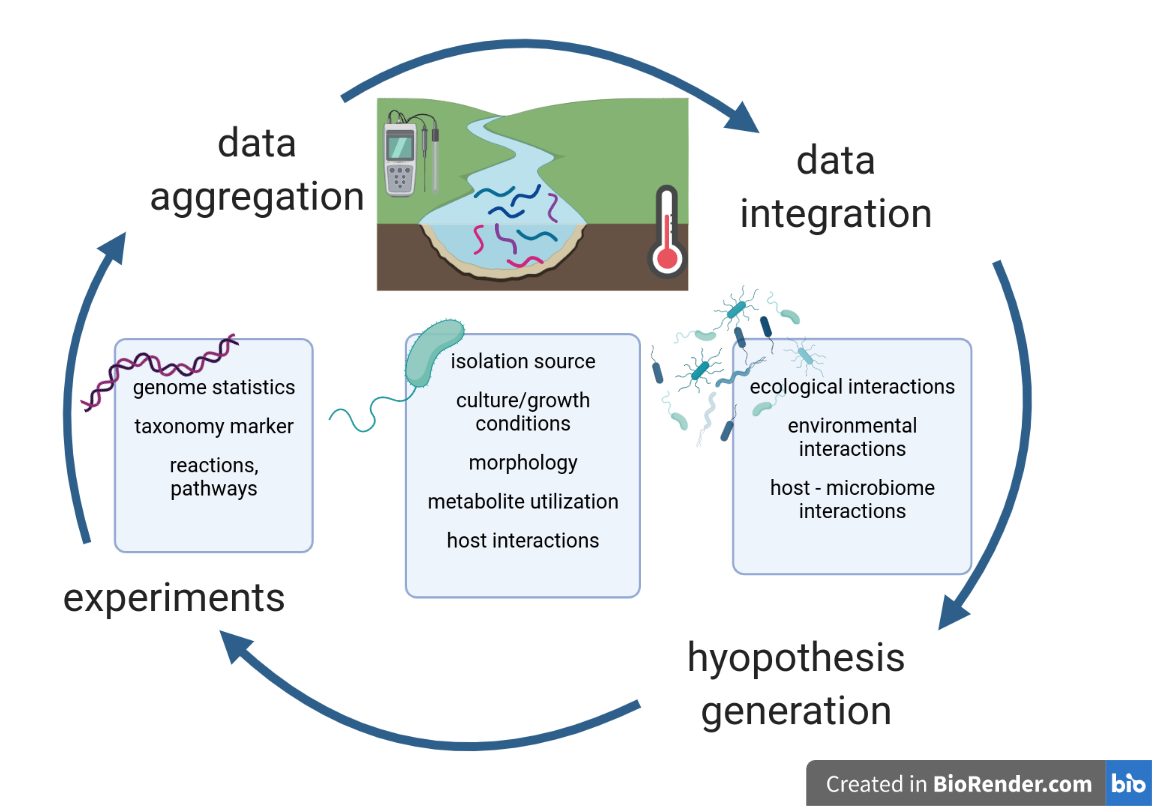
\includegraphics[width=0.95\textwidth]{figures/data_integration_scheme.png}
         \caption[Data integration in Microbial Ecology]{A data integration scheme for microbial ecology oriented data. 
         Measurements from experiments at every level of organization of life are gathered and their summary provides researchers with new insight. Created with \href{BioRender.com}{BioRender.com}.
         }
         \label{fig:data_int}
      \end{figure}


      One of the most typical examples of data integration and its potential
      is the \href{https://www.string-db.org/}{STRING database}\footnote{\href{https://www.string-db.org/}{https://www.string-db.org/}}, where multiple channels of information are combined 
      to retrieve protein - protein interactions~\cite{mering2003string, szklarczyk2021string}. 
      In addition to databases of interaction experiments and others of interaction predictions, text-mining methods of the scientific literature enhance further the 
      PPI predictions~\cite{szklarczyk2021string}.
      Focusing on bacterial information, \href{https://bacdive.dsmz.de/}{BacDive}\footnote{\href{https://bacdive.dsmz.de/}{https://bacdive.dsmz.de/}}~\cite{reimer2019bac}
      is a great example - resource of the added value that data integration methods can provide. 

      \paragraph{Multiple integration approaches} attempt to address the challenges described. 
      The \textit{data warehousing} approach is a widely used data integration approach and has two mains steps; 
      first, a unified data model that can accommodate all types of  
      information from the various source databases is schemed.
      Then, software is developed aiming at  
      gathering the data from the source databases, 
      convert them to match the unified data model and 
      then load them into the warehouse~\cite{stein2003integrating}.
      Once these steps have been completed, further analysis of the once
      several bits of information - now a single dataset, can be performed.
      New insight may come up either from statistical analyses on the unified
      dataset or from their visualization~\cite{leonelli2013integrating}.  

      

   \subsection{Ontologies \& metadata standards}

      Data integration in general, 
      is strongly dependent by the extent that standards are used. 
      Especially in case of vast and heterogeneous data, 
      data integration cannot return valid results 
      when there is not a certain way
      of denoting the entities included.
      Thus, it is dependent on the way data are distributed in the fist place 
      as well as on whether their content follow certain principles or not. 
      To address these challenges, several ontologies and standards have 
      been established through the years, trying to cover all the different 
      types of needs of the microbial ecology community. 

      According to~\citeauthor{stevens2000ontology} an \textit{ontology} is the \textit{"concrete form of a concepcualisation
      of a community's knowledge of a domain"}~\cite{stevens2000ontology}.
      Ontologies attempt to capture the main concepts in a \textit{knowledge domain}, 
      i.e. a body of knowledge that is often associated with a
      specialized scientific discipline. 
      For example, considering \textit{where} a species live or \textit{where} a process occurs, one need to describe the environment where the phenomeno under study 
      takes place. 
      Thus, the \href{https://sites.google.com/site/environmentontology}{Environment Ontology (ENVO)}\footnote{\href{https://sites.google.com/site/environmentontology}{https://sites.google.com/site/environmentontology}} aims to provide descriptions of environments~\cite{buttigieg2016environment}.
      Using sets of entities, meaning entities sharing several attributes (\textit{concepts}), 
      descriptions of the interactions between concepts (\textit{relations}), 
      entities - members of a concept (\textit{instances}) and 
      properties of relations that aim to constrain the value a class or an instance may get (\textit{axioms}) aim to create an agreed vocabulary and
      semantic structure for exchanging
      information about that domain~\cite{stevens2000ontology}. 
      A \textit{vocabulary} includes definitions and an indication of how concepts are inter-related which collectively impose a structure on the domain and constrain the
      \cite{uschold1998enterprise}.
      Ontologies are fundamental for data integration as they ensure that the knowledge
      inclduded in a text or in a data set, can be captured by both humans and computers. 


      \paragraph{Metadata are fundamental} for all types of data. 
      Consider sampling patients without knowing who is sick and who is not. 
      As discussed in Section~\ref{subsec:hts_chal}


      Metadata standard definition: minimum set and formats (Some flexibility will have to be considered in sharing standards between domain-specific communities).
      Systems to extract the vast amount of metadata locked in the scientific literature and provide them in standard format (explored by the Biodiversity Focus Group).






      \cite{stevens2000ontology}


      \if 0 

      To define biome - feature - material, have a look a this
      https://www.ddbj.nig.ac.jp/faq/en/biome-feature-material-e.html

      \fi



      The Community initially focused on developing open science "best practices" for the research community. 
      The paper "The metagenomic data life-cycle: standards and best practices" \citep{ten2017metagenomic} provided the foundation for FAIR data management in the domain. 
      These best practices advocated using community standards for contextual provenance and metadata at all stages of the research data life cycle.



      For the ENA, extensive documentation exists on how to submit data which both encourages compliance with metadata standards and provides separate submission guidelines for different data types - usage of the documentation can mitigate common errors and often aid first-time submitters but does not reach the full user-base. 

      FAIR principles, to provide a multilayer set of metadata required by the different scientific communities, reflecting the inherently multi-disciplinary character of environmental microbiology. 


      \if 0
      \begin{figure}[!h]
         \centering
         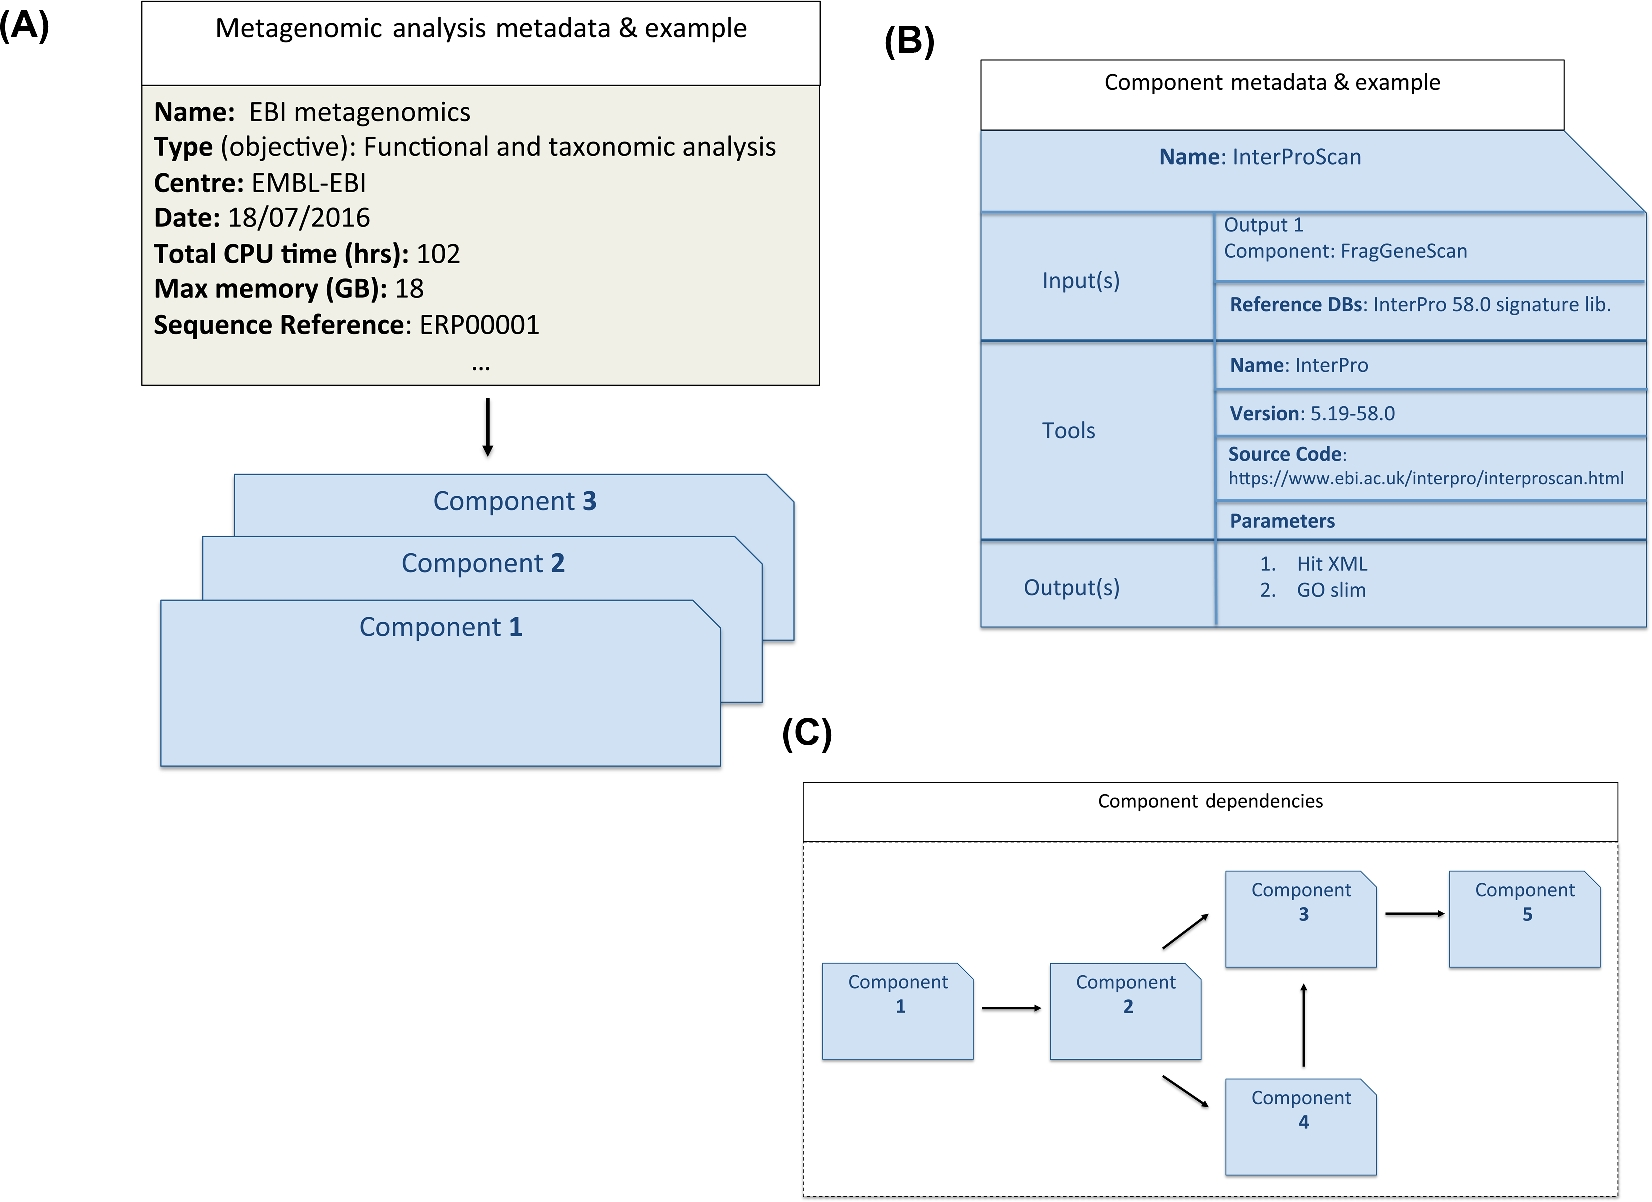
\includegraphics[width=.95\textwidth]{figures/metadata_Scheme.jpeg}
         \caption[Metadata collection for metagenomic data]{
            Schematic overview of best practice for analysis metadata collection with example fields. 
            A) Overarching metadata; 
            B) Analysis component; 
            C) Workflow. 
            Figure from~\cite{ten2017metagenomic} under 
            \href{http://creativecommons.org/licenses/by/4.0/}{Creative Commons Attribution License}
            }
         \label{fig:metadata}
      \end{figure}
      \fi


      \begin{figure}[!h]
         \hspace*{-0.9in}
         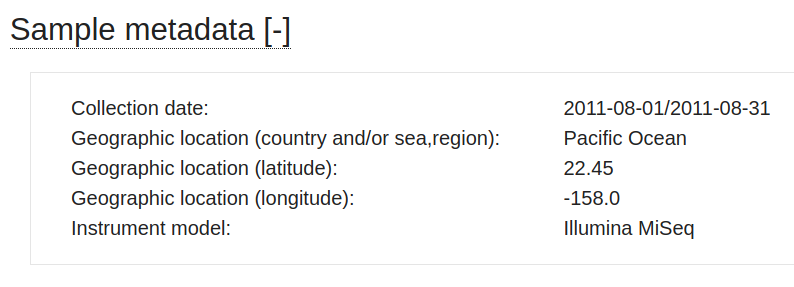
\includegraphics[width=.7\textwidth]{figures/SRS1753450_metadata.png}
         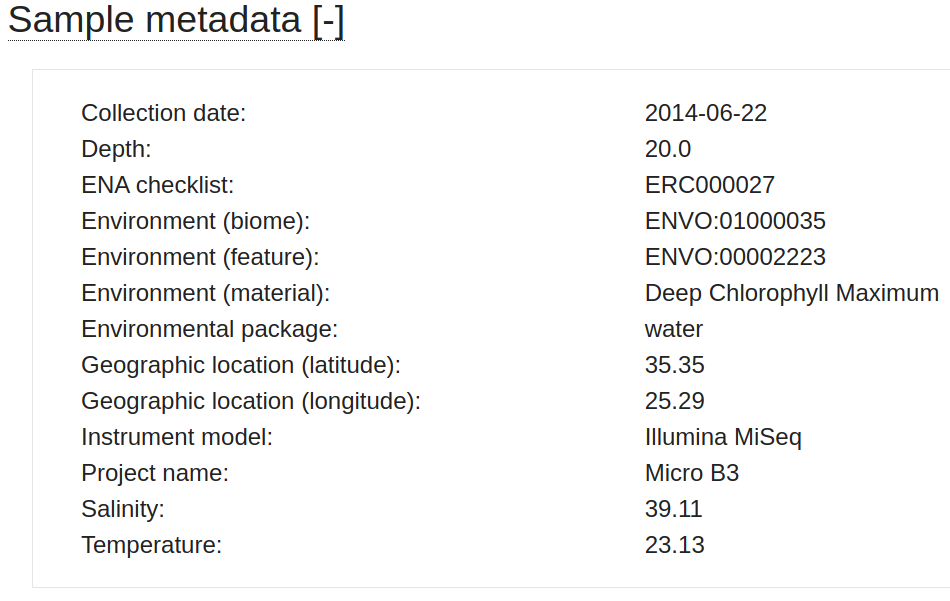
\includegraphics[width=.7\textwidth]{figures/ERS667566_metadata.png}
         \caption[Samples metadata examples MGnify]{Bad and not perfect example}
         \label{fig:metadata_examples}
      \end{figure}



      The various layers of metadata necessary for the FAIRification of MAGs should include:
      \begin{enumerate}
         \item Environmental data describing the sample of origin
         \item Sequencing technology or technologies
         \item Details on the computational pipeline for metagenome assembly, binning and quality assessment
         \item Connection to an existing taxonomy schema
      \end{enumerate}


      OSD’s open access strategy and provenance for metadata annotation is reflected in its ENA and Pangea submissions. 
      Among others Standardization and training are key aspects across OSD: from sampling protocols to metadata checklists and guidelines. 
      This is inline with aims of the Elixir microbiome community (see Sections "Mobilising raw data and metadata", 
      "Training - lack of training"); 
      spreading the experience to other biomes can benefit such ends.




   

      \if 0

      \begin{itemize}
         \item Metadata of the cleaned data; metadata associated with the data sequencing, sample collection (MIMS), and quality control analyses and the workflow
         \item Metadata of the assembled data
         \item Metadata to accompany the taxonomic inventories

      \end{itemize}  


      Databases

      \begin{itemize}
         \item GenBank, ENA
         \item repositories such as MGnify 
         \item PubMed
      \end{itemize}


      Ontologies: 

      \begin{itemize}
         \item ENVO
         \item NCBI Taxonomy 
         \item Gene Ontology 
         \item Uniprot
         \item KEGG
         \item https://edamontology.org/page
      \end{itemize}
      \fi

      Only by a concerted effort on the part of the database providers, and with the encouragement and support of the research community, will we be able to tame the explosion of biological data



\section{Metabolic networks: modeling  cellular physiology and growth}


   \subsection{Reverse ecology: transforming ecology into a high-throughput field}

      % - genotype - phenotype relationship \\
      Chapter 15
      Reverse Ecology: From Systems
      to Environments and Back

      \begin{figure}[!h]
         \centering
         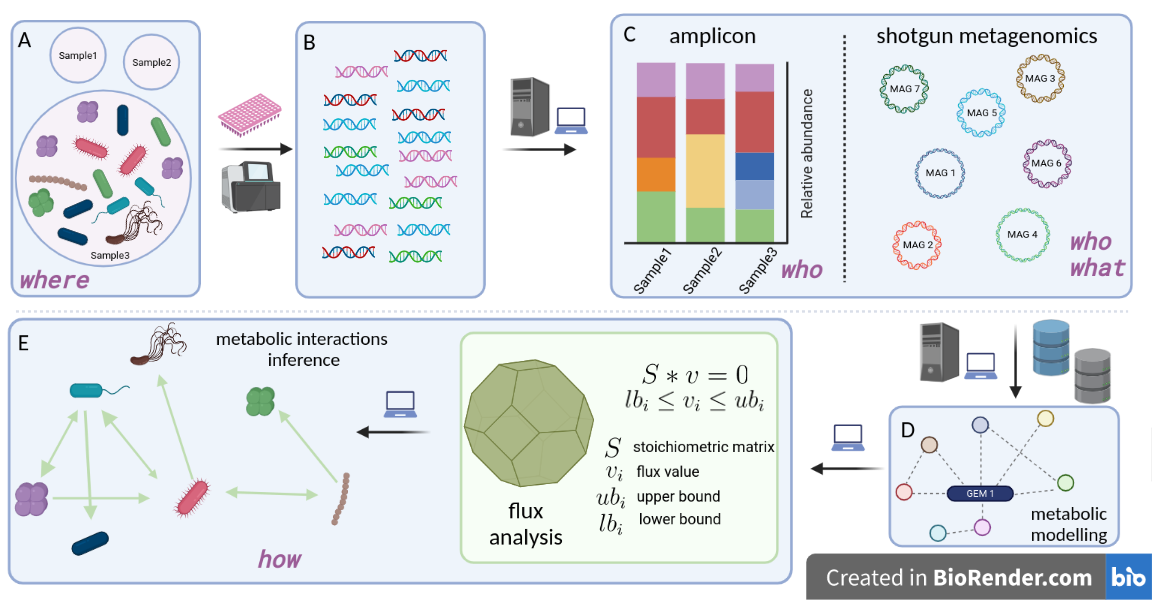
\includegraphics[width=135mm]{figures/reverse_ecology.png}
         \caption[The \textit{Reverse Ecology} framework.]{The \textit{Reverse Ecology} framework. Without any previous knowledge of the species present in a community (A) and using HTS data (B) one can have an overview of the species present 
         as well as in the functional profile of the community (C).
         Especially when the complete genome of a species has been retained (either using 
         metagenomics (MAG) or using targeted approaches to get this (SAG))
         reseachers can build its corresponding GEM (D) and then 
         infer the ecology of a taxon predicting 
         the exogenously acquired compounds as well as ecological interactions between the taxon under study and other species present in a community (E). 
         Both network topology - and constraint - based methods can be used to this end.
         Created with \href{BioRender.com}{BioRender.com}.
         }
         \label{fig:revecol}
      \end{figure}

      \if 0 

      (from Roie Levy and Elhanan Borenstein~\cite{levy2012reverse})
      Reverse Ecology—an emerging new frontier in Evolutionary Systems Biology—aims
      to extract this information and to obtain novel insights into an organism’s ecology.
      The Reverse Ecology framework facilitates the translation of high-throughput
      genomic data into large-scale ecological data, and has the potential to transform
      ecology into a high-throughput field


      the traditional approach taken to studies relating genetics and ecology:
      first an ecological adaptive phenotype is identified, then various methodologies are
      employed to detect causal genetic variation.






      In some cases, however, one may wish to predict not only potential interactions
      but also specific metabolic dynamics in a community of microorganisms and the
      exact set of metabolites being exchanged actively between the various species. The
      prediction of specific metabolic fluxes is mostly beyond the scope of topology-
      based metabolic models and requires a more involved modeling framework such
      as constraint-based modeling (CBM) [18, 19]. Such models, however, are usually
      limited in scale and require detailed and manually curated data [20].







      (from RevEcoR publication~\cite{cao2016revecor})
      A systematic approach for describing microbiome ecologies and the interactions between microbiota is lacking. 
      To address this challenge, a systems biology approach called \textit{reverse ecology} has been developed 
      to study the complex interactions and species composition of microbial communities [4]. 
      Reverse ecology uses genomics to study community ecology with no a priori assumptions about the organisms under consideration. 
      Researchers can use it to infer the ecology of a system directly from genomic information. 
      The reverse ecology framework uses advances in systems biology and genomic metabolic modeling and 
      the system-level analysis of complex biological networks to predict the ecological traits of poorly studied microorganisms, 
      their interactions with other microorganisms, and the ecology of microbial communities. 
      Several studies have applied this approach to investigate the interactions between microorganisms 
      and their surroundings on a large scale [4, 5].

      The relationship between genotype and phenotype is fundamental to biology.
      Many levels of control are introduced when moving from one to the other. 
      Systems biology aims at deciphering "the strategy" both at the cell and at higher levels of organization, in case of multicell species, that enables organisms to produce orderly adaptive behavior in the face of widely varying genetic and environmental conditions (\cite{strohman2002maneuvering}); 
      the term "strategy" is used as per \cite{polanyi1968life}.
      Systems biology approaches aim at interpreting how a system's properties emerge; 
      from the cell to the community level.
      As \citeauthor{polanyi1968life} (\citeyear{polanyi1968life}) underlines 
      "live mechanisms and information in DNA are boundary conditions with a sequence of boundaries above them". 




      Being at the helm of the most critical celular functions  
      metabolism and therefore, metabolic networks and their analysis, 
      play a key role in Systems Biology. 
      Moreover, \citeauthor{lewis2012constraining} (\citeyear{lewis2012constraining}) 
      describe thoroughly the multiple constraint-based reconstruction and analysis (COBRA) methods 
      that have been developed to support the analysis of such networks. 


      % SUPERS SOS !!! 
      The modeling frameworks and topology-based analyses discussed above are a
      powerful toolbox for analyzing potential metabolic dependencies between species.
      In some cases, however, one may wish to predict not only potential interactions
      but also specific metabolic dynamics in a community of microorganisms and the
      exact set of metabolites being exchanged actively between the various species. The
      prediction of specific metabolic fluxes is mostly beyond the scope of topology-
      based metabolic models and requires a more involved modeling framework such
      as constraint-based modeling (CBM) [18, 19]. 





   \subsection{Sampling the flux space of a metabolic model: challenges \& potential}



   \fi



% SECTION 7 - first draft ready
\section{Aims and objectives}

   The aim of this PhD was double:
   \begin{enumerate}
      \item to enhance the analysis of microbiome data by building algorithms and software 
            to address some of the on-going computational challenges on the field.
      \item to exploit these methods to identify taxa, functions, especially related to sulfur cycle, 
            and microbial interactions that support life in microbial community assemblages in hypersaline sediments.
   \end{enumerate}
   All parts of this work are purely computational. 
   Samples and their corresponding sequencing data used in Chapter~\ref{cha:swamp} have been collected 
   and produced by \href{https://scholar.google.com/citations?user=3zs1rNkAAAAJ&hl=en&oi=sra}{Dr. Christina Pavloudi}. 

   In \textbf{Chapter~\ref{cha:2}}, challenges derived from the analysis of HTS amplicon data are examined.
   A bioinformatics pipeline, called \texttt{PEMA}, for the analysis of several marker genes was developed, combinining several new technologies that allow large scale analysis of hundreds of samples. 
   In addition, a software tool called \texttt{darn}, was built to investigate the unassigned sequences in amplicon data of the COI marker gene. 

   In \textbf{Chapter~\ref{cha:prego}}, data integration, data mining and text-mining methods were exploited to build a knowledge-base, called \texttt{prego}, including millions of associations between:
   \begin{enumerate}
      \item microbial taxa and the environments they have been found in 
      \item microbial taxa and biological processes they occur
      \item environmental types and the biological processes that take place there
   \end{enumerate}

   In \textbf{Chapter~\ref{cha:dingo}}, the challenges of flux sampling in metabolic models of high dimensions was presented along with a Multiphase Monte Carlo Sampling (MMCS) algorithm we developed. 

   In \textbf{Chapter~\ref{cha:hpc}}, the history of the IMBBC-HCMR HPC facility was presented indicating the vast needs of computing resources in modern analyses in general and in microbial studies more specifically. 

   In \textbf{Chapter~\ref{cha:swamp}}, sediment samples from a hypersaline swamp in Tristomo, Karpathos Greece were analysed using both amplicon and shotgun metagenomics. 
   The taxonomic and the functional profiles of the microbial communities present there were investigated. 
   Key metabolic processes for ensuring life at such an extreme environment were identified.
   Microbial interactions of the assemblages retrieved were also studied by exploiting 
   data integration and reverse ecology approaches.  


   Finally, in \textbf{Chapter~\ref{cha:conclusion}}, general discussion and conclusions that have derived from this research were presented. 





% -------------------------
%    NOTES
% -------------------------
% 
%    biotic interactions                  --> cross-feeding of byproduscts, competition for nutrients 
%    confounder (or 'confounding factor') --> something, other than the thing being studied, that could be causing the results seen in a study. 
%                                             confounders have the potential to change the results of research because they can influence the outcomes
%                                             that the researchers are measuring.
%                                             EXAMPLE: we found that people eating red meat have higher possibility for heart issues; but we have to 
%                                                      check whether everyone in the study who ate a lot of red meat may also have smoked cigarettes
%                                                      regularly or been overweight. 
%    circumvented                         --> shortchut, find a way around (an obstacle).
%    stratify                             --> stromatopoio // 
%    stringent                            --> austiros, strict
%    a habitat filtering model supposes that
% habitats with differing environmental
% features support non-overlapping sets of taxa
